%%%%%%%%%%%%%%%%%%%%%%%%%%%%%%%%%%%%%
\section{Protocol: SADS}
%%%%%%%%%%%%%%%%%%%%%%%%%%%%%%%%%%%%%

When \emph{streaming authenticated data structure (SADS)} is used, analytic server and web servers can update its own digest independently from each other.  
Therefore, web servers are able to maintain a small digest only, instead of maintaining a whole SADS tree.

The protocol can be used for any case of single or multiple web servers.
If multiple web servers participate in the protocol, client is assumed to know IP addresses of all participating web servers. 
Analytic server is assumed to maintain one SADS per each web server. 
However, maintaining only one SADS for multiple web servers is also possible, since digests of web servers can be summed up at verification by client due to its homomorphic property.

Since analytic data is transmitted to analytic server and web server, two servers should be always synchronized to prevent (or minimize) inconsistency. 
In this context, \emph{2-phase commit} protocol is proposed for transmission of analytic data. 
This protocol also makes inconsistencies between analytic server and web servers reconcilable. 
Once a user's web browser receives the analytic Javascript, it collects analytic data from the user's machine and sends the analytic data with IP address of the web server to analytic server. 
Analytic data is sent as parameters of HTTP request for a small gif (Google Analytics) or PHP (Piwik) files. 
Therefore the web browser is able to determine if the transmission of analytic data is successful or not. 
If the transmission to the analytic server is unsuccessful, a user's web browser terminates the protocol immediately and may restart the protocol. 
The analytic server defers updating its SADS until it receives confirm message from the user's web browser. 
If successful, the user's web browser sends the analytic data to the web server. 
Receiving analytic data from, the web server updates its digest. 
If transmissions to both web server and analytic server are successful, then the user's web browser sends confirm message to analytic server and it updates SADS.

In this protocol, an inconsistency between the web server and the analytic server can arise only when confirm message to analytic server is not delivered successfully. 
Therefore the protocol guarantees that web server always have all the analytic data confirmed by analytic server. 
This provides a basis for reconciliation process described in \ref{label:reconcile}.

The overall protocol is depicted in Figure \ref{fig:sads}.

\begin{figure}
        \centering
        \begin{subfigure}[t]{0.49\textwidth}
                \centering
                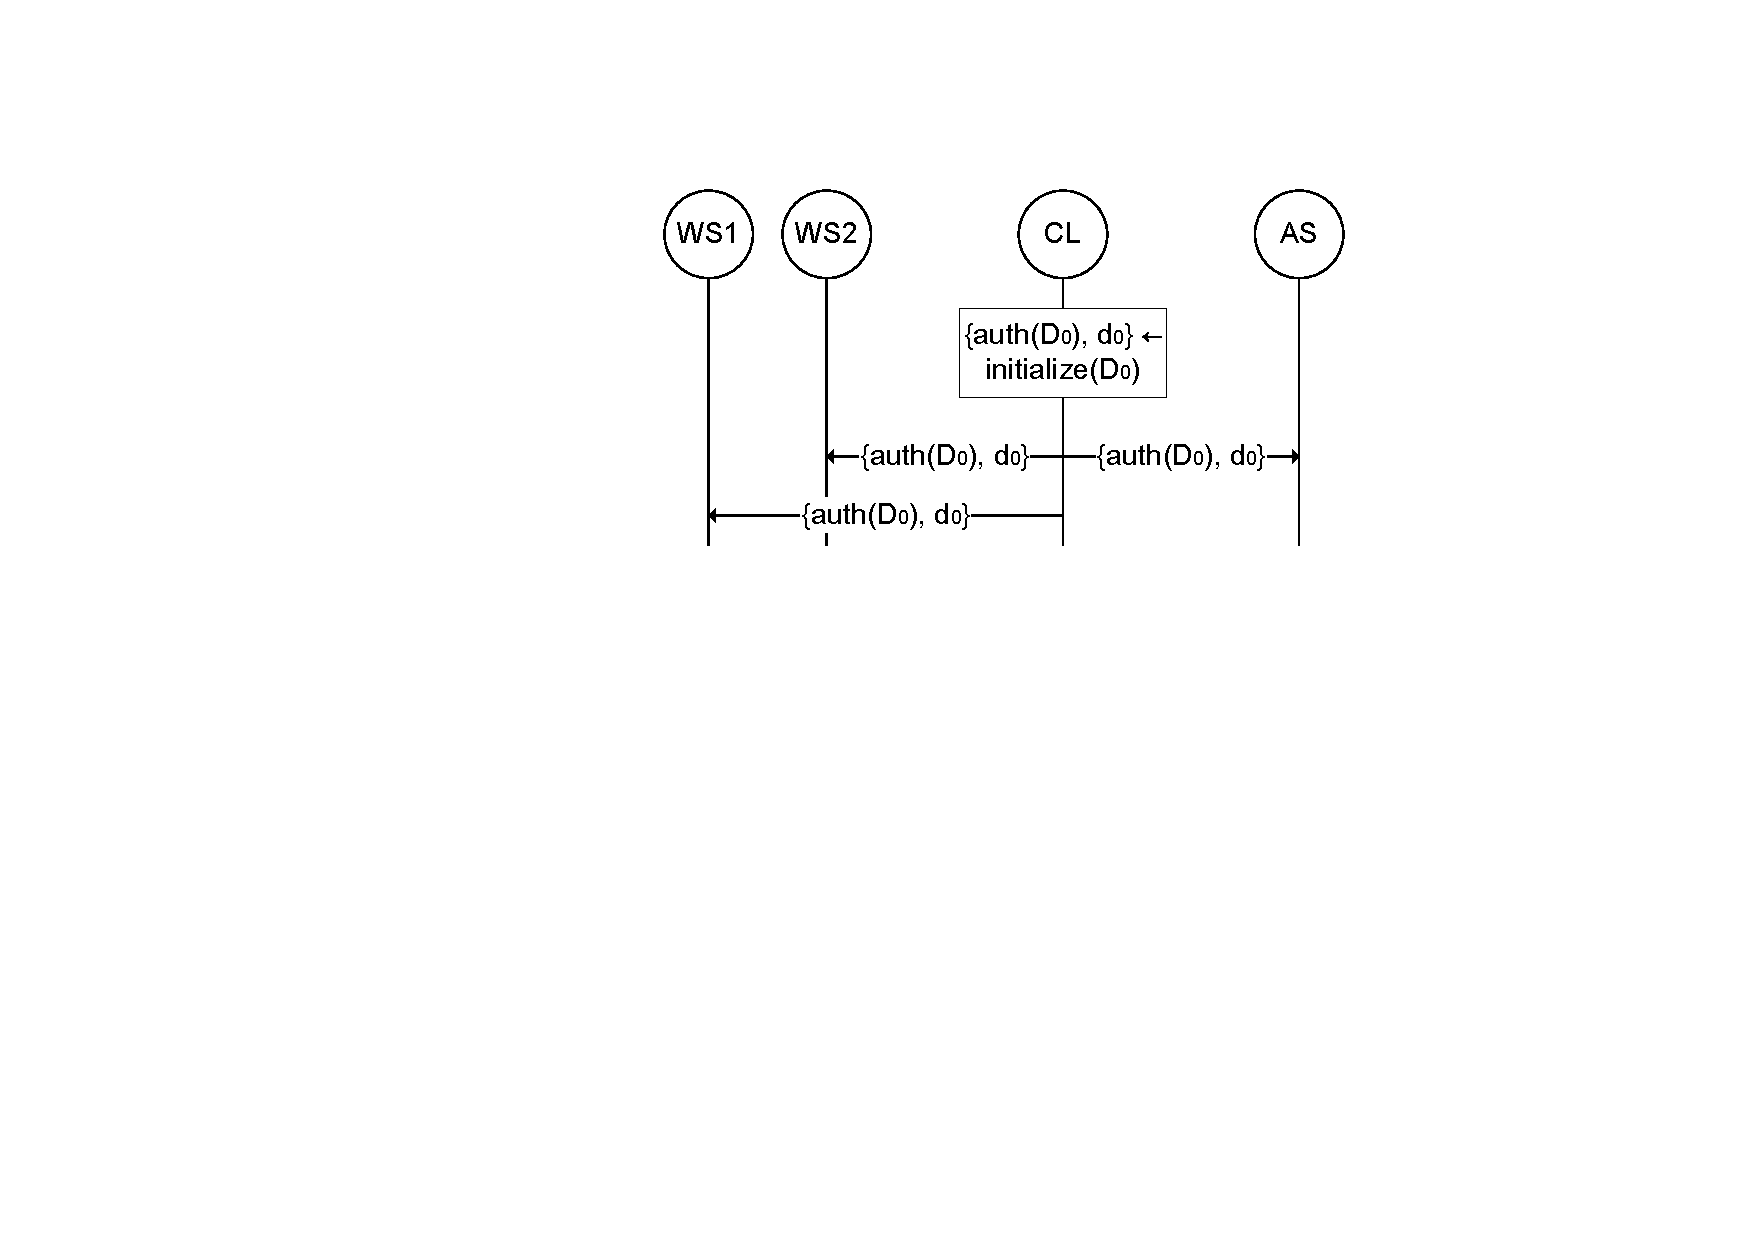
\includegraphics[width=\textwidth]{figure/sads_1.pdf}
                \caption{initialize()}
                \label{fig:sads_1}
        \end{subfigure}
        \begin{subfigure}[t]{0.49\textwidth}
                \centering
                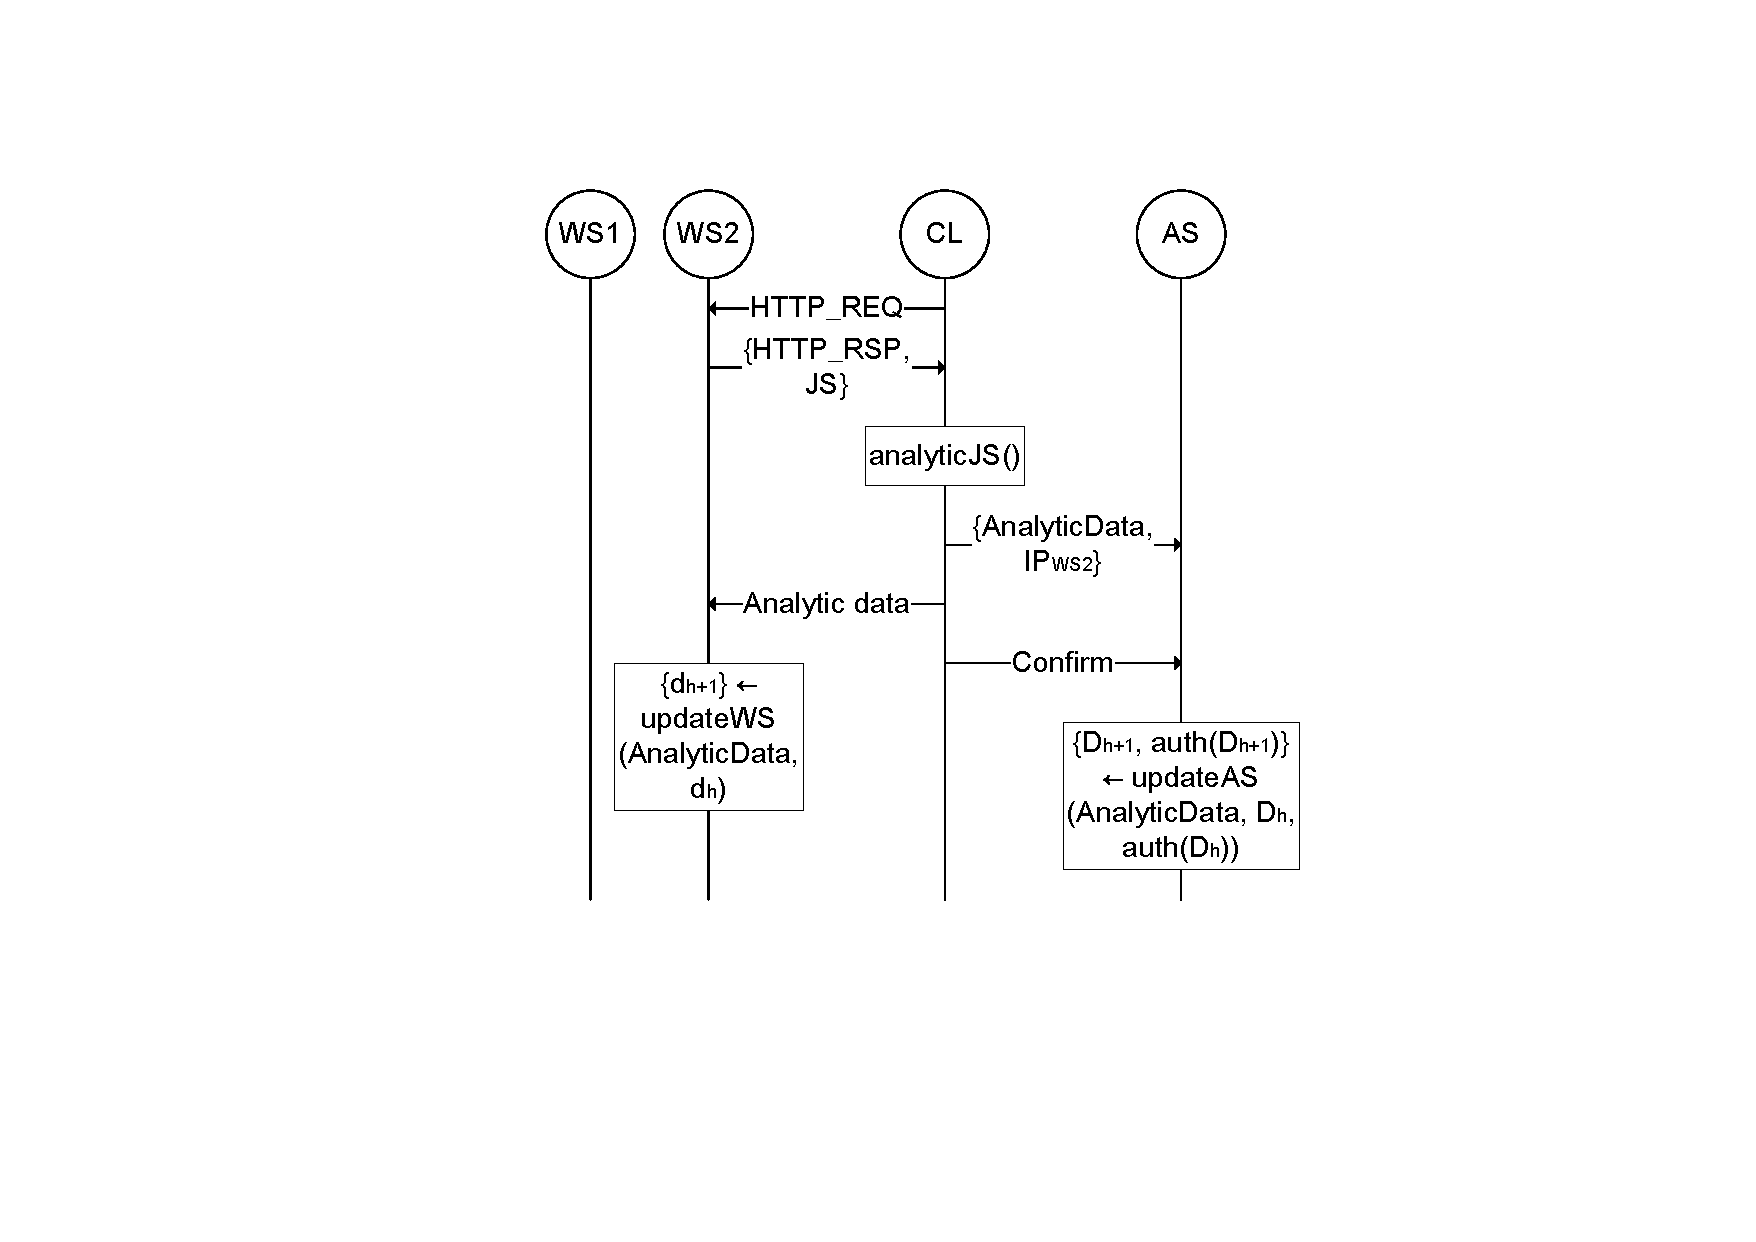
\includegraphics[width=\textwidth]{figure/sads_2.pdf}
                \caption{2-Phase commit}
                \label{fig:sads_2}
        \end{subfigure}

        ~ %add desired spacing between images, e. g. ~, \quad, \qquad etc.
          %(or a blank line to force the subfigure onto a new line)
	\newline

        \begin{subfigure}[t]{0.49\textwidth}
                \centering
                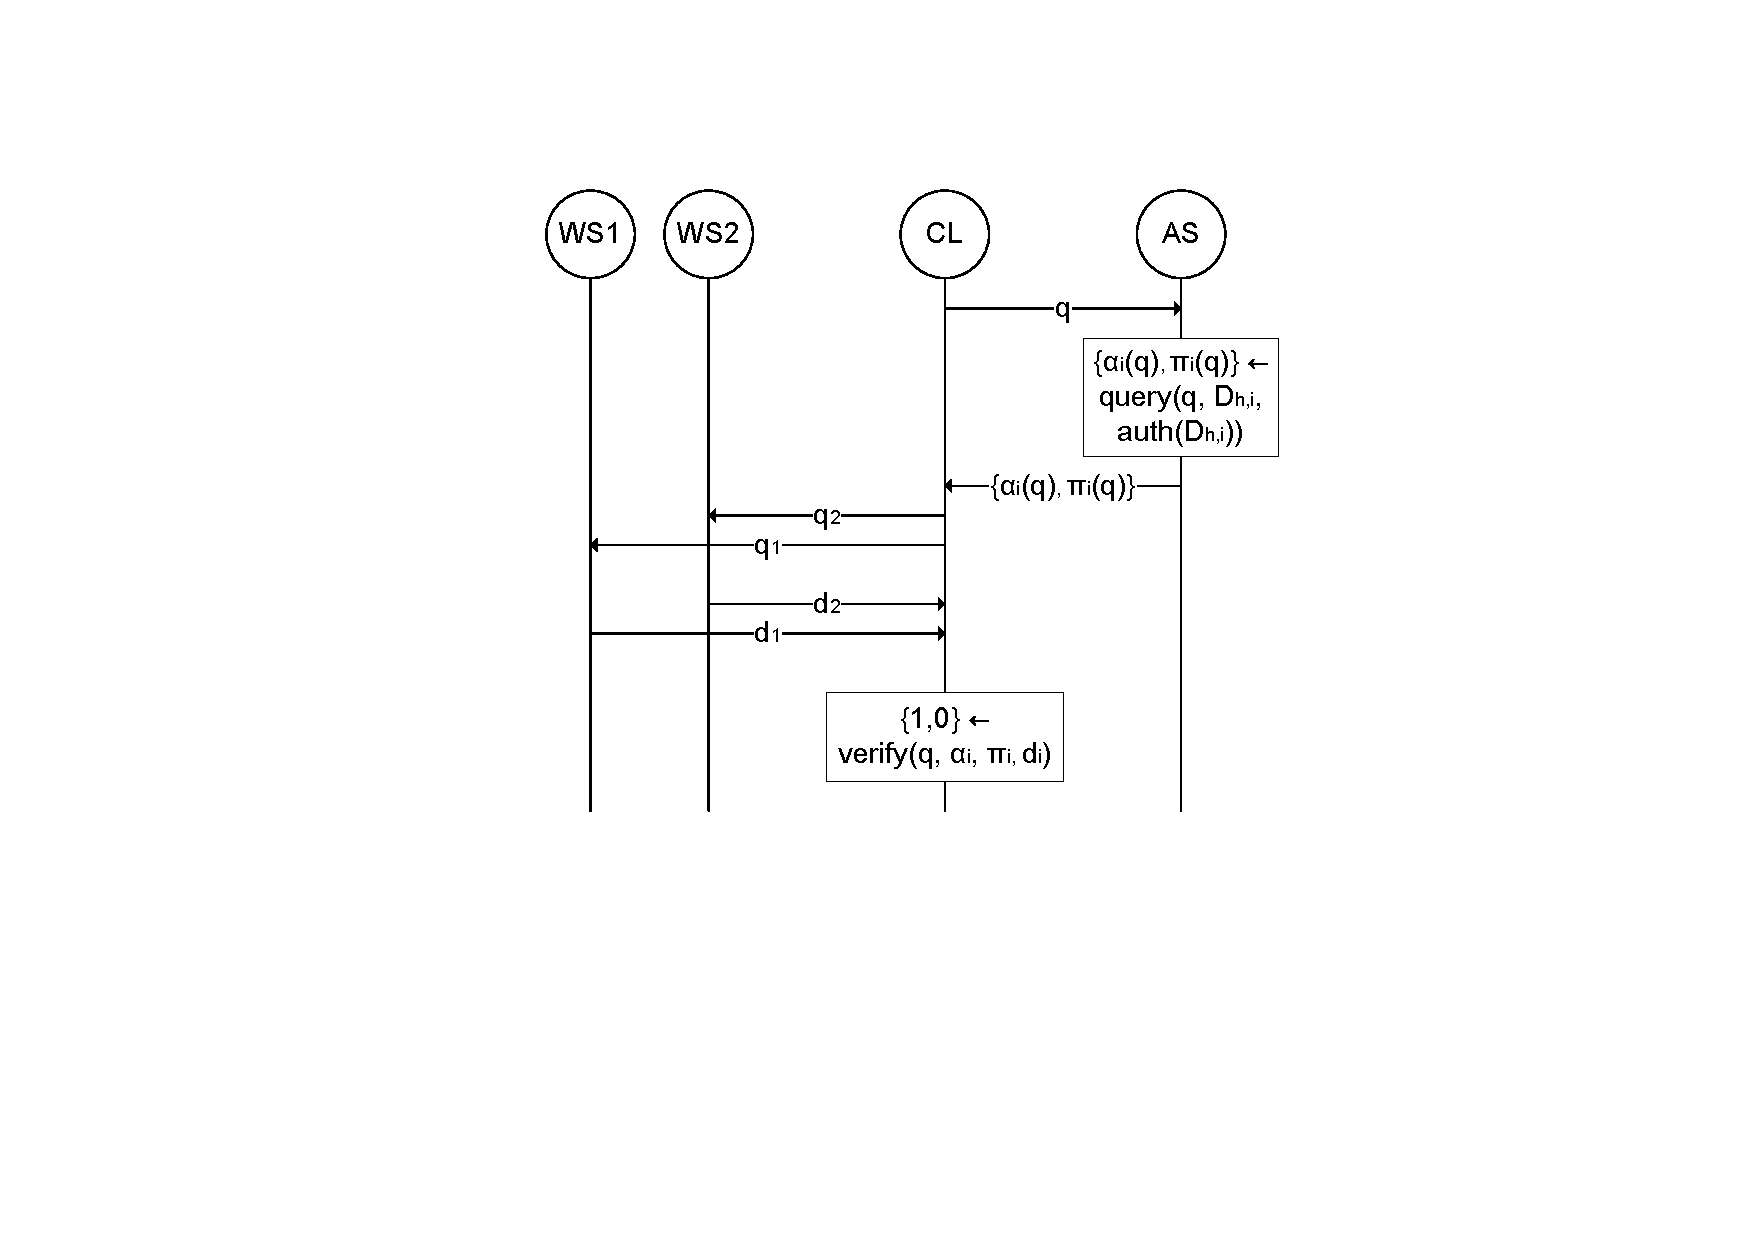
\includegraphics[width=\textwidth]{figure/sads_3.pdf}
                \caption{query() and verify()}
                \label{fig:sads_3}
        \end{subfigure}
        \begin{subfigure}[t]{0.49\textwidth}
                \centering
                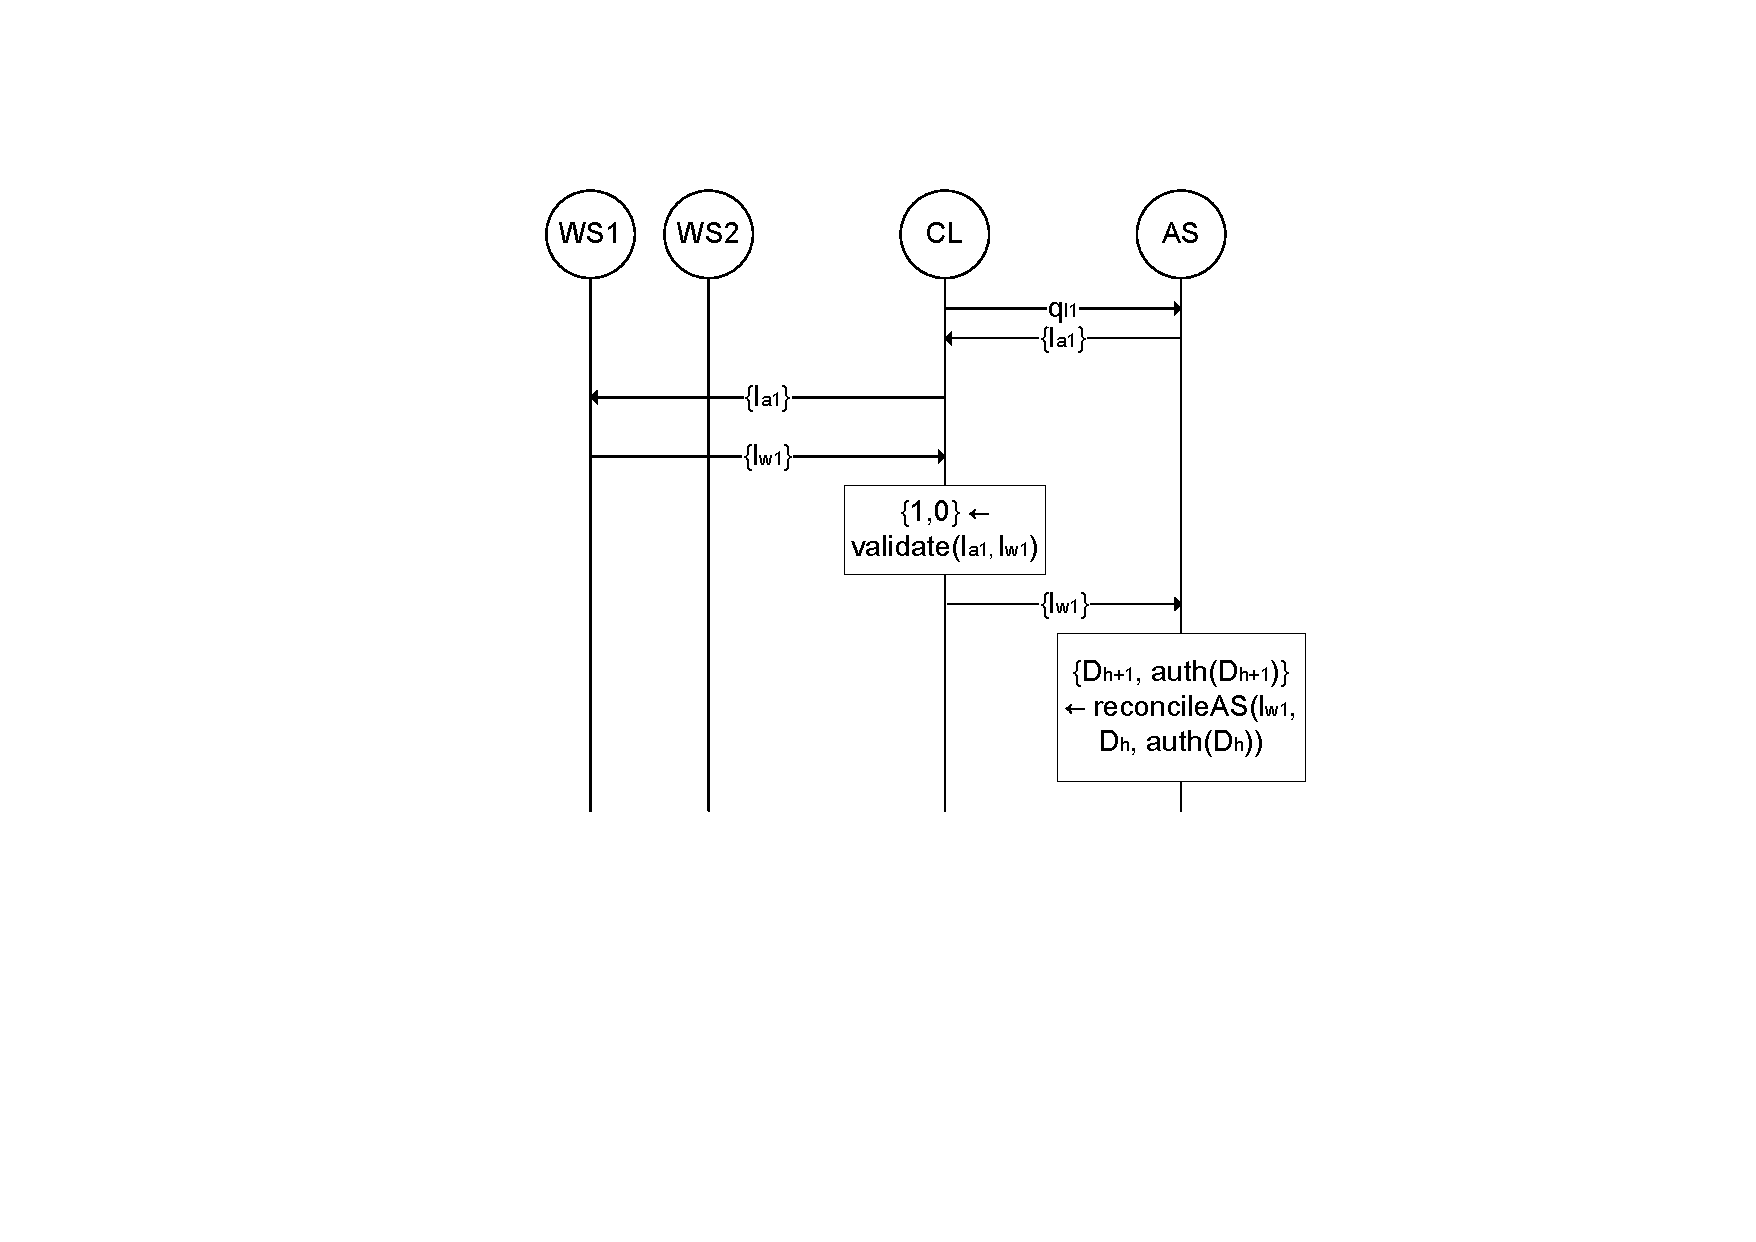
\includegraphics[width=\textwidth]{figure/sads_4.pdf}
                \caption{reconcile()}
                \label{fig:sads_4}
        \end{subfigure}
        \caption{Protocol w/ SADS}
	\label{fig:sads}
\end{figure}

%%%%%%%%%%%%%%%%%%%%%%%
% initialize
%%%%%%%%%%%%%%%%%%%%%%%
\subsection{Initialization}

\begin{framed}
\noindent
\textbf{CL}: \textsf{ \{auth($D_0$), $d_0$\} $\leftarrow$ initialize($D_0$)}	\\
\textbf{CL $\rightarrow$ AS}: \textsf{ \{auth($D_0$), $d_0$\} } 	\\
\textbf{CL $\rightarrow$ WS}: \textsf{ \{auth($D_0$), $d_0$\} } 	\\
\line(1,0){450}

\noindent
Let $D_0$ be an initial empty dictionary.  \textsf{initialize()} outputs SADS \textsf{auth($D_0$)} and its digest \textsf{$d_0$}.
Client \textsf{CL} sends \textsf{\{auth($D_0$), $d_0$\}} to analytic server \textsf{AS} and web servers \textsf{WS$_i$} ($\forall i$, $i = \{1,...,N_{ws}\}$ where $N_{ws}$ is the number of web servers hosting the web site). 
\end{framed}


%%%%%%%%%%%%%%%%%%%%%%%
% AnalyticData collection
%%%%%%%%%%%%%%%%%%%%%%%
\subsection{Analytic data collection}
\begin{framed}
\noindent
\textbf{WB $\rightarrow$ WS$_i$}: \textsf{\{HTTP\_REQ\}}	\\
\textbf{WS$_i$ $\rightarrow$ WB}: \textsf{\{HTTP\_RSP, JS\}}	\\
\textbf{WB}: \textsf{\{AnalyticData\} $\leftarrow$ analyticJS()}	\\
\line(1,0){450}

\noindent
A user's web browser \textsf{WB} sends \textsf{HTTP\_REQ} to \textsf{WS$_i$} to access the web site.
\textsf{WS$_i$} transmits \textsf{HTTP\_RSP} with analytic Javascript \textsf{JS} to \textsf{WB}.
Then \textsf{WB} collects \textsf{AnalyticData} by running received analytic Javascript code \textsf{analyticJS()}.
\end{framed}


%%%%%%%%%%%%%%%%%%%%%%%
% 2-Phase commit
%%%%%%%%%%%%%%%%%%%%%%%
\subsection{Update: 2-Phase commit}
\label{label:2phase_commit}

\begin{framed}
\begin{enumerate}
\item{1st Phase}\\
\textbf{WB $\rightarrow$ AS}: \textsf{\{AnalyticData, IP$_{WS_i}$\}}	\\
\textbf{WB $\rightarrow$ WS}: \textsf{\{AnalyticData\}}	\\
\textbf{WS}: \textsf{\{$d_{h+1}$\} $\leftarrow$ updateWS(AnalyticData, $d_h$)}	

\item{2nd Phase}\\
\textbf{WB $\rightarrow$ AS}: \textsf{\{Confirm\}}	\\
\textbf{AS}: \textsf{\{$D_{h+1}$, auth($D_{h+1}$)\} $\leftarrow$ updateAS(AnalyticData, $D_h$, auth($D_h$))}
\end{enumerate}
\line(1,0){450}

\noindent
\textsf{WB} sends \textsf{AnalyticData} with IP address of \textsf{WS$_i$} \textsf{IP$_{WS_i}$} to \textsf{AS}. 
If succeed, \textsf{WB} sends \textsf{AnalyticData} to \textsf{WS}. 
\textsf{WS} performs \textsf{updateWS()} which outputs an updated digest \textsf{$d_{h+1}$}. \\
If the 1st phase is performed successfully, \textsf{WB} sends a confirmation message \textsf{Confirm} to \textsf{AS}. 
Then \textsf{AS} performs \textsf{updateAS()} which outputs an updated dictionary \textsf{$D_{h+1}$} and SADS \textsf{auth($D_{h+1}$)}.
\end{framed}

%%%%%%%%%%%%%%%%%%%%%%%
% query
%%%%%%%%%%%%%%%%%%%%%%%
\subsection{Query}
\begin{framed}
\noindent
\textbf{CL $\rightarrow$ AS}: \textsf{\{$q$\}}	\\
\textbf{AS}: \textsf{\{$\alpha(q)$, $\Pi(q)$\} $\leftarrow$ query($q$, $D_h$, auth($D_h$))}	\\
\textbf{AS $\rightarrow$ CL}: \textsf{\{$\alpha(q)$, $\Pi(q)$\}}	\\

\noindent
\textbf{CL $\rightarrow$ WS}: \textsf{\{$q_{d}$\}}	\\
\textbf{WS $\rightarrow$ CL}: \textsf{\{$d$\}}	\\
\line(1,0){450}

\noindent
Let $\alpha(q)$ denote an answer to a query $q$ and $\Pi(q)$ denote a proof of the answer $\alpha(q)$. 
Query $q$ can be either membership or range query. 
\textsf{CL} sends a query $q$ to \textsf{AS}. 
Upon receiving $q$, \textsf{AS} performs \textsf{query()} and outputs \textsf{\{$\alpha(q)$, $\Pi(q)$\}}.
Then \textsf{AS} sends \textsf{\{$\alpha(q)$, $\Pi(q)$\}} to \textsf{CL}.

\noindent
On the other hand, \textsf{CL} sends a query $q_d$ to \textsf{WS} to request a digest $d$. 
\textsf{WS} sends its digest \textsf{$d$} to \textsf{CL}.
\end{framed}

%%%%%%%%%%%%%%%%%%%%%%%
% verify
%%%%%%%%%%%%%%%%%%%%%%%
\subsection{Verification}
\begin{framed}
\noindent
\textbf{CL}: \textsf{\{0, 1\} $\leftarrow$ verify($q$, $\alpha(q)$, $\Pi(q)$, $d$)}	\\
\line(1,0){450}

\noindent
\textsf{CL} performs \textsf{verify()} to check if $\alpha(q)$ and $\Pi(q)$ is authenticated correctly and the digest derived from $\Pi(q)$ matches to $d$ received from the web server.
\textsf{verify()} outputs $1$ if \textsf{\{$\alpha(q)$, $\pi(q)$\}} are proved to be authenticated correctly and otherwise, outputs $0$.
\end{framed}

%%%%%%%%%%%%%%%%%%%%%%%
% reconcile
%%%%%%%%%%%%%%%%%%%%%%%
\subsection{Reconciliation}
\label{label:reconcile}

\begin{framed}
\noindent
\textbf{CL $\rightarrow$ AS}: \textsf{\{$q_{\ell}$\}}		\\
\textbf{AS $\rightarrow$ CL}: \textsf{\{$\ell_a$\}}		\\

\noindent
\textbf{CL $\rightarrow$ WS}: \textsf{\{$\ell_a$\}}		\\
\textbf{WS $\rightarrow$ CL}: \textsf{\{$\ell_w$\}}		\\

\noindent
\textbf{CL}: \textsf{\{0,1\}} $\leftarrow$ \textsf{validate($\ell_a$, $\ell_w$)}		\\

\noindent
\textbf{CL $\rightarrow$ AS}: \textsf{\{$\ell_w$\}}		\\
\textbf{AS}: \textsf{\{$D_{h+1}$, auth($D_{h+1}$)\} $\leftarrow$ reconcileAS($\ell_w$, $D_h$, auth($D_h$))}	\\
\line(1,0){450}

\noindent
Let $q_\ell$ denote a query requesting the list of \textsf{AnalyticData} $\ell_a$ that are not paired with \textsf{Confirm} message from \textsf{AS}.
If \textsf{verify()} outputs $0$, \textsf{CL} sends $q_\ell$ to \textsf{AS} and receives $\ell_a$ from \textsf{AS}.
Then \textsf{CL} forwards $\ell_a$ to \textsf{WS}.
\textsf{WS} selects from $\ell_a$ the list of \textsf{AnalyticData} that were actually received.
Then \textsf{WS} generates $\ell_w$, a sublist of \textsf{$\ell_a$}, and sends it back to \textsf{CL}.

\noindent
\textsf{CL} performs \textsf{validate()} to check if the current inconsistency between \textsf{AS} and \textsf{WS} is recoverable. 
\textsf{validate()} outputs $1$ if $(|\ell_a| - |\ell_w| < Threshold )$ and $0$ otherwise.  
If the inconsistency is reconcilable, \textsf{CL} sends $\ell_w$ to \textsf{AS}, and \textsf{AS} performs \textsf{reconcileAS()} which outputs updated \textsf{\{$D$, auth($D$)\}}

\end{framed}



%%%%%%%%%%%%%%%%%%%%%%%%%%%%%%%%%%%%%
\section{Protocol: Merkle Hash Tree}
%%%%%%%%%%%%%%%%%%%%%%%%%%%%%%%%%%%%%

If \emph{Merkle hash tree} is used as the authenticated data structure, both analytic server and web servers should maintain Merkle hash trees since updating digest without interaction between web servers and analytic server is not possible. 
We can try to sync two Merkle hash trees to maintain the size of trees as small as possible but it doesn't change the fact that web servers should always maintain its own Merkle hash tree. 
So using Merkle hash tree in this project seems to be inefficient in terms of space and computation of \textsf{WS}.

As in the protocol with SADS, analytic server maintains one Merkle hash tree per each web server. 
However, Merkle hash trees of web servers can be merged into a single Merkle hash tree at query time. 
Therefore, analytic server may maintain only one Merkle hash tree if web servers maintain their own Merkle hash trees.

The overall protocol is depicted in Figure \ref{fig:merkle}.

\begin{figure}
        \centering
        \begin{subfigure}[t]{0.495\textwidth}
                \centering
                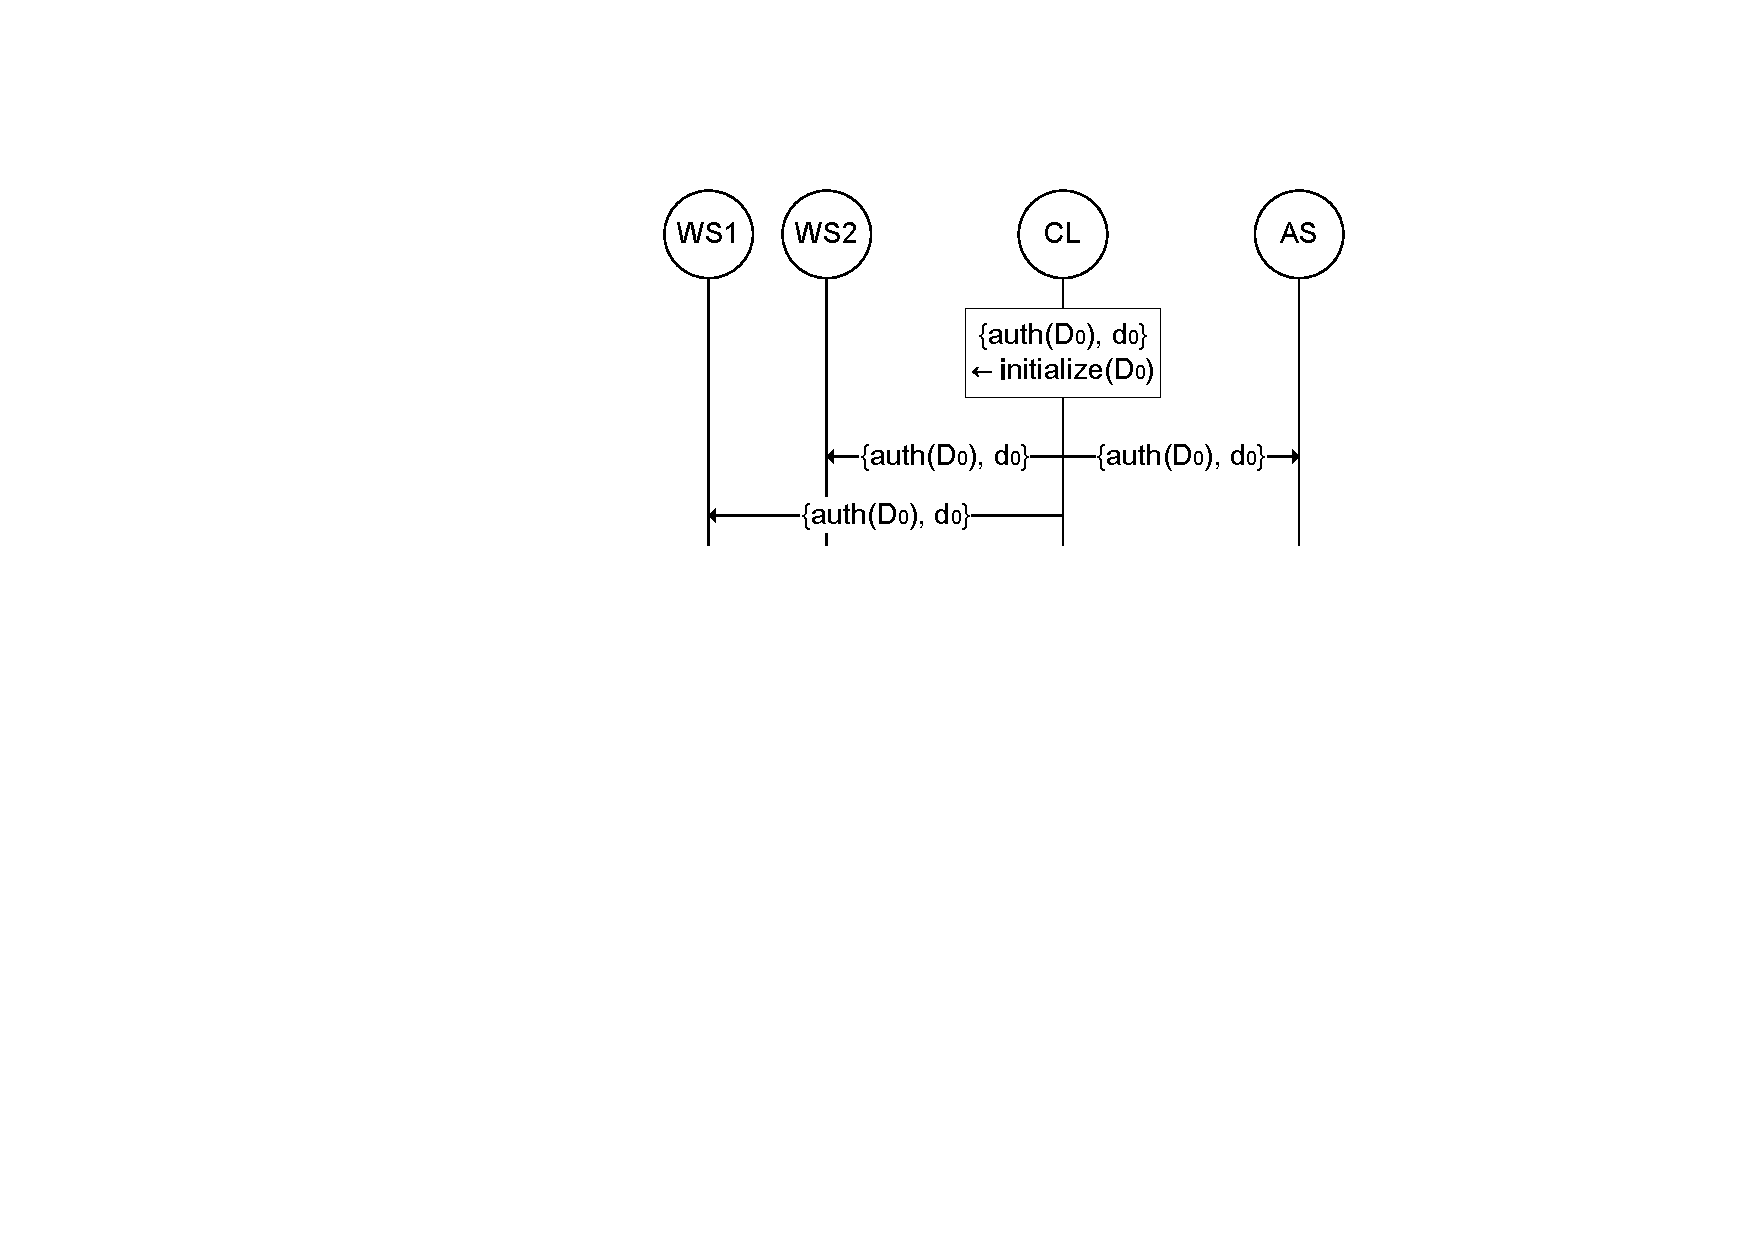
\includegraphics[width=\textwidth]{figure/merkle_1.pdf}
                \caption{initialize()}
                \label{fig:merkle_1}
        \end{subfigure}%
        ~ %add desired spacing between images, e. g. ~, \quad, \qquad etc.
          %(or a blank line to force the subfigure onto a new line)
        \begin{subfigure}[t]{0.495\textwidth}
                \centering
                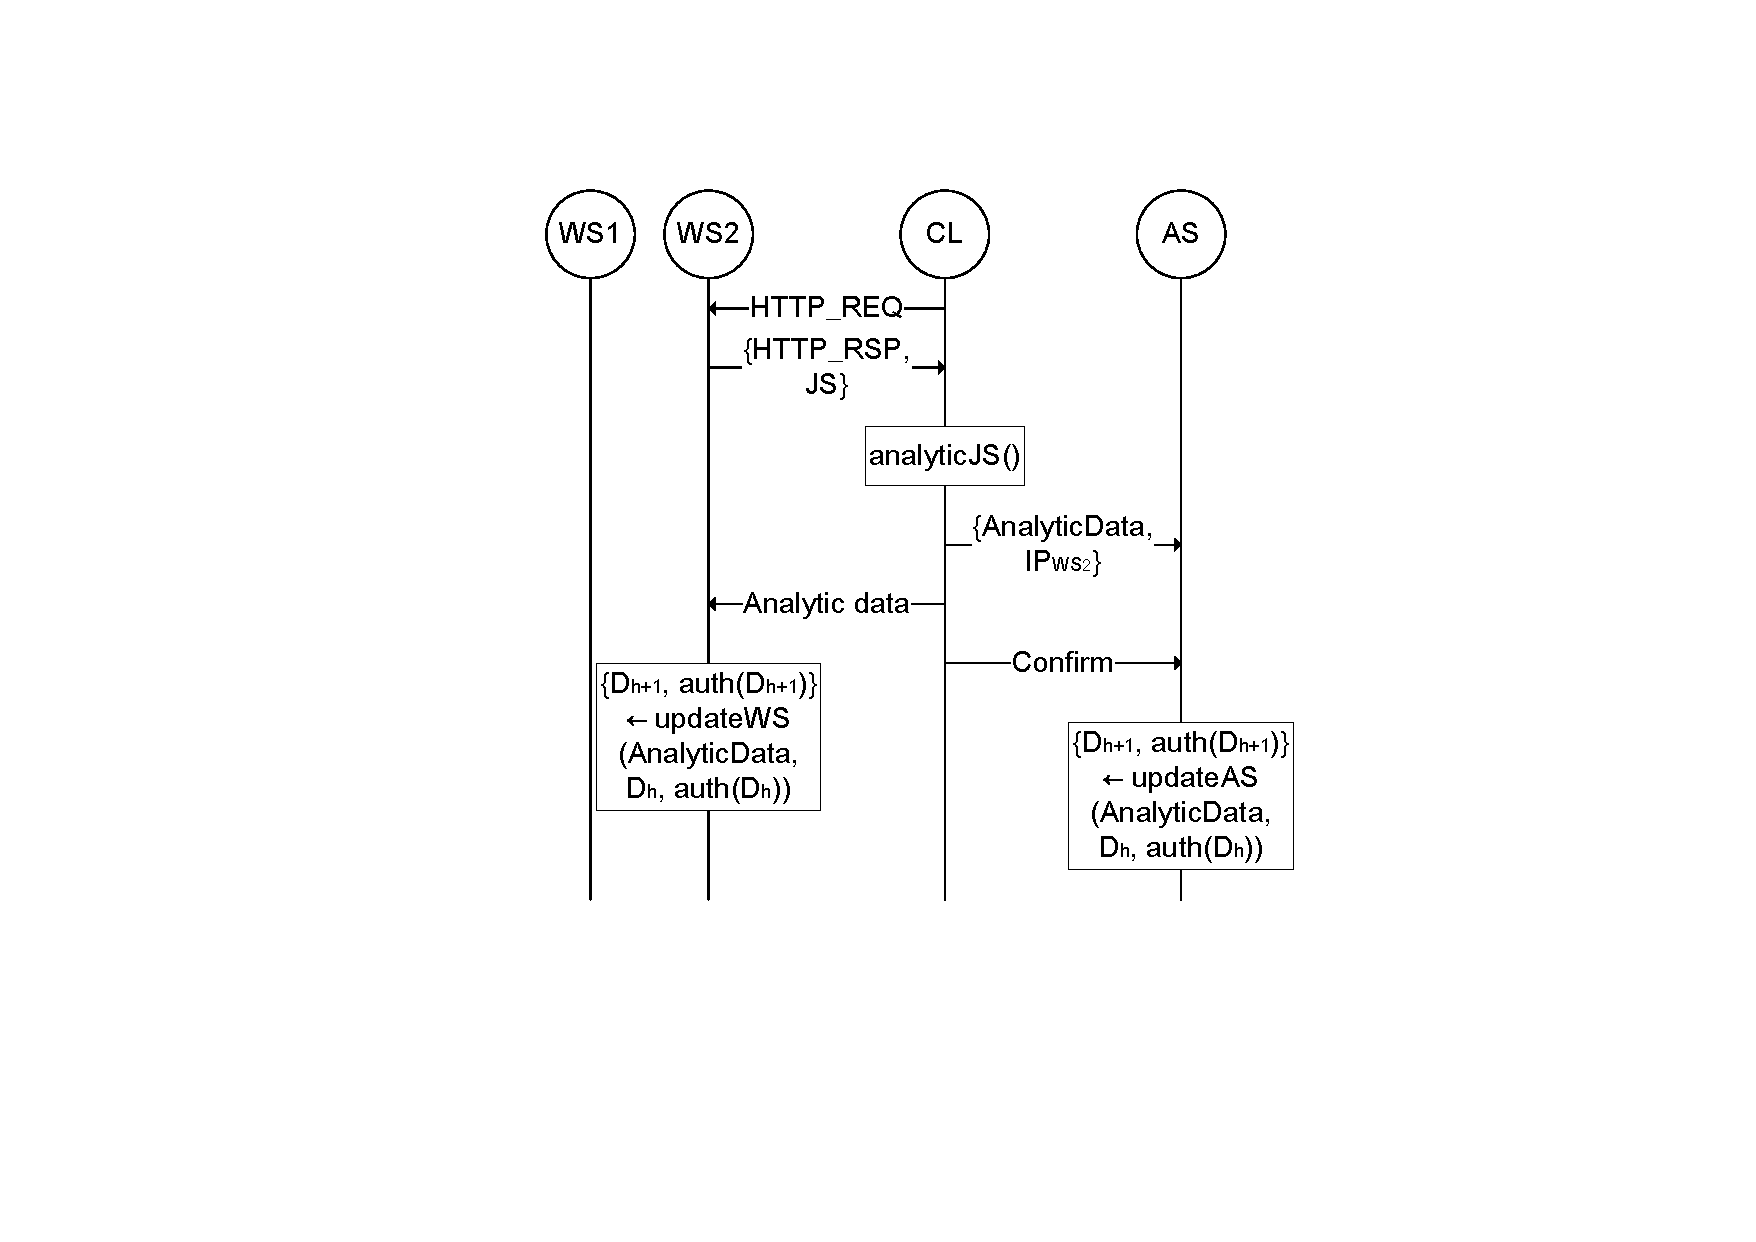
\includegraphics[width=\textwidth]{figure/merkle_2.pdf}
                \caption{2-Phase commit}
                \label{fig:merkle_2}
        \end{subfigure}
	\newline

        \begin{subfigure}[t]{0.495\textwidth}
                \centering
                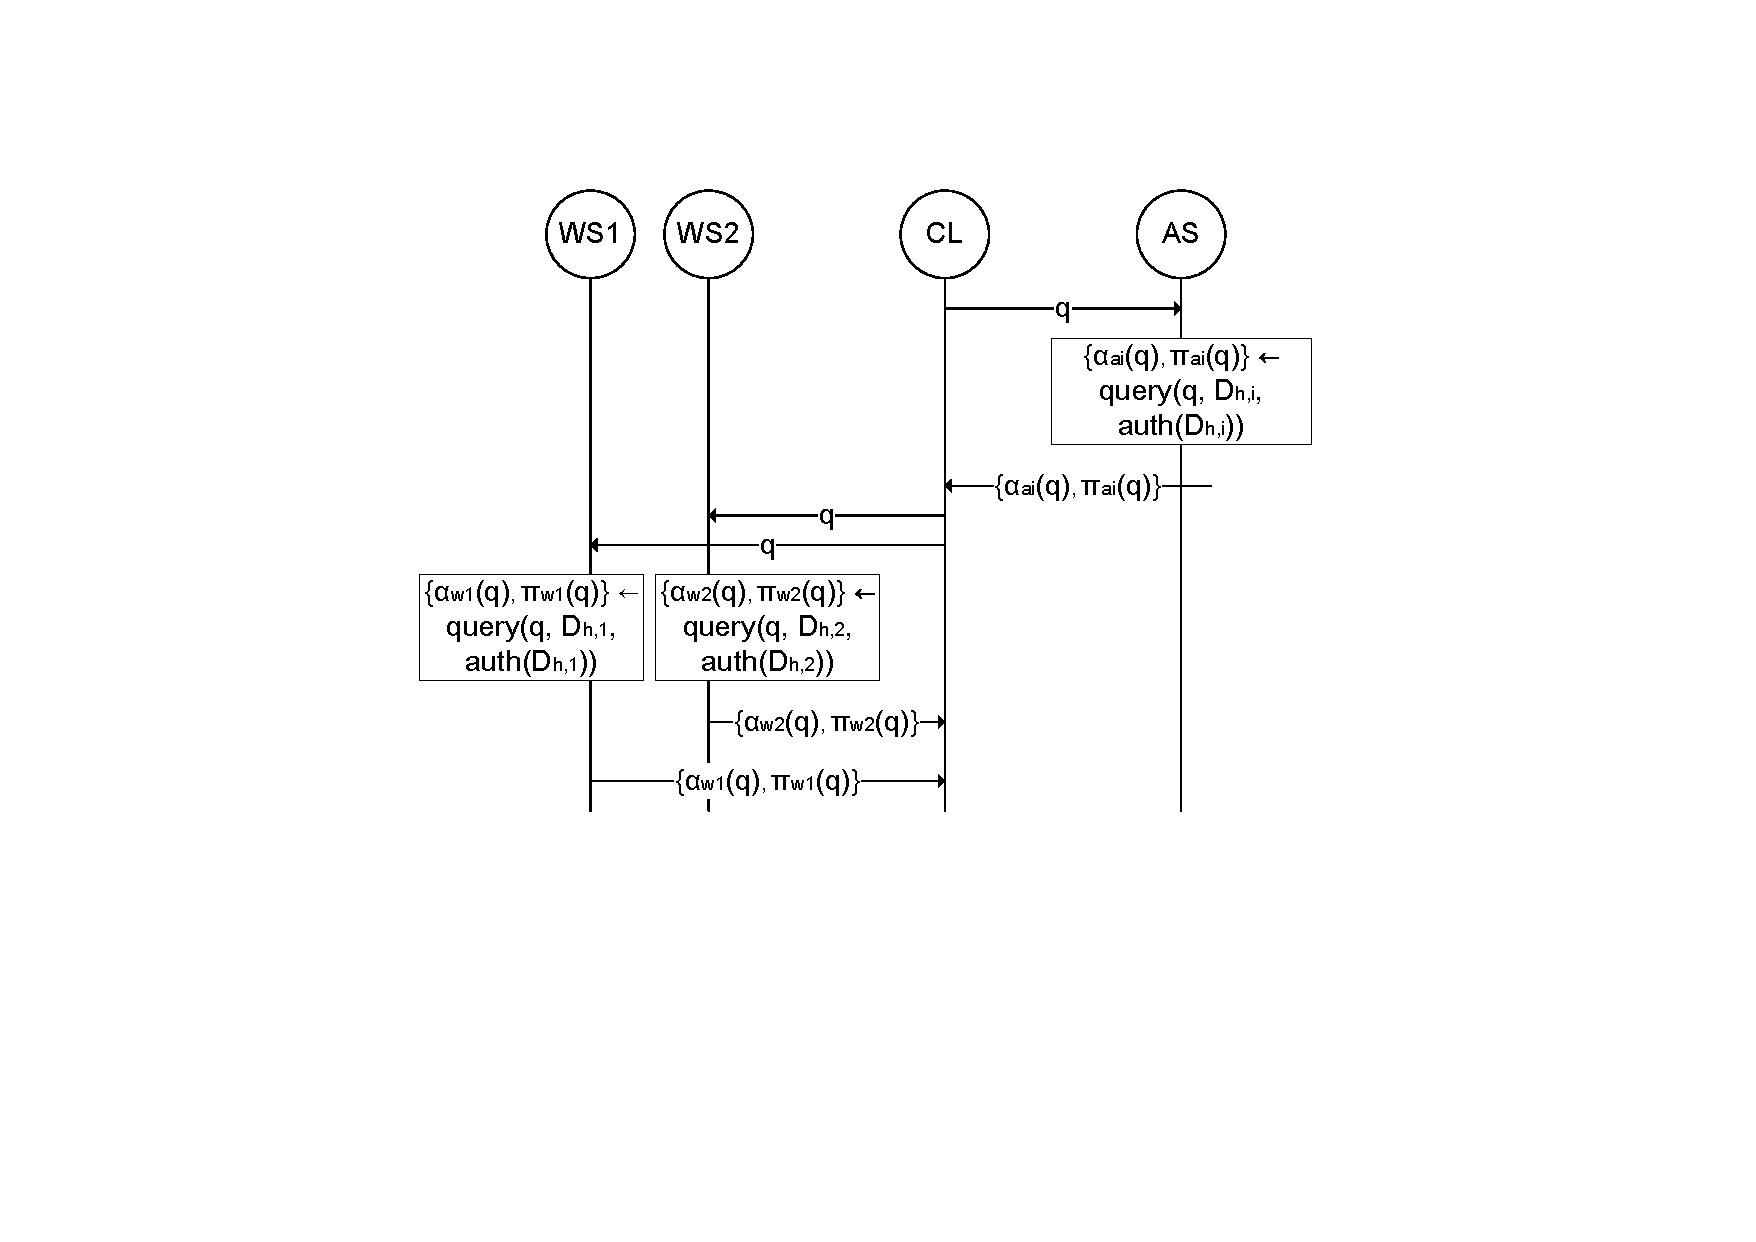
\includegraphics[width=\textwidth]{figure/merkle_3.pdf}
                \caption{query() and verify()}
                \label{fig:merkle_3}
        \end{subfigure}
        \begin{subfigure}[t]{0.495\textwidth}
                \centering
                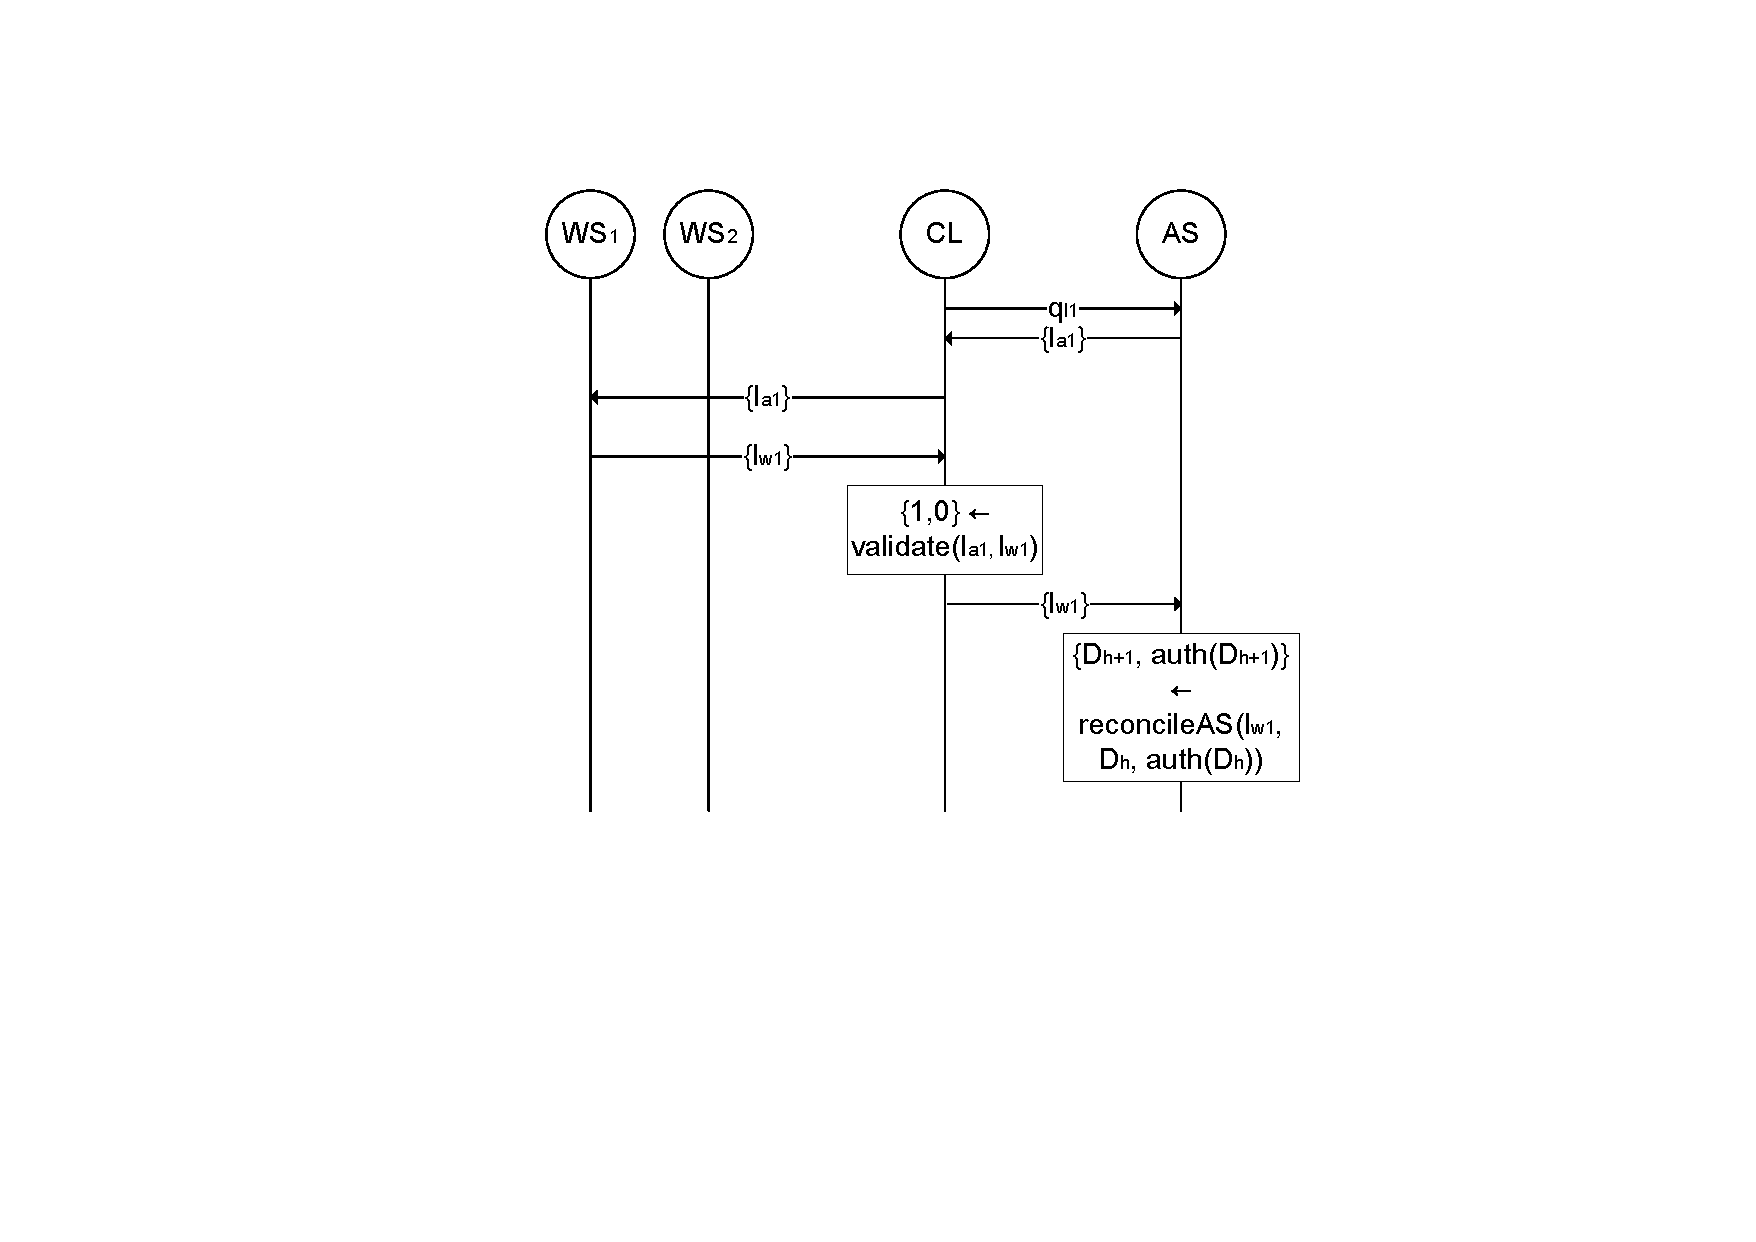
\includegraphics[width=\textwidth]{figure/merkle_4.pdf}
                \caption{reconcile()}
                \label{fig:merkle_4}
        \end{subfigure}
        \caption{Protocol w/ Merkle Hash Tree}
	\label{fig:merkle}
\end{figure}


%%%%%%%%%%%%%%%%%%%%%%%
% initialize
%%%%%%%%%%%%%%%%%%%%%%%
\subsection{Initialization}

\begin{framed}
\noindent
\textbf{CL}: \textsf{ \{auth($D_0$), $d_0$\} $\leftarrow$ initialize($D_0$)}	\\
\textbf{CL $\rightarrow$ AS}: \textsf{ \{auth($D_0$), $d_0$\} } 	\\
\textbf{CL $\rightarrow$ WS}: \textsf{ \{auth($D_0$), $d_0$\} } 	\\
\line(1,0){450}

\noindent
Let $D_0$ be an initial empty dictionary.  \textsf{initialize()} outputs Merkle hash tree \textsf{auth($D_0$)} and its digest \textsf{$d_0$}.
Client \textsf{CL} sends \textsf{\{auth($D_0$), $d_0$\}} to analytic server \textsf{AS} and web servers \textsf{WS$_i$} ($\forall i$, $i = \{1,...,N_{ws}\}$ where $N_{ws}$ is the number of web servers hosting the web site). 
\end{framed}


%%%%%%%%%%%%%%%%%%%%%%%
% AnalyticData collection
%%%%%%%%%%%%%%%%%%%%%%%
\subsection{Analytic data collection}
\begin{framed}
\noindent
\textbf{WB $\rightarrow$ WS$_i$}: \textsf{\{HTTP\_REQ\}}	\\
\textbf{WS$_i$ $\leftarrow$ WB}: \textsf{\{HTTP\_RSP, JS\}}	\\
\textbf{WB}: \textsf{\{AnalyticData\} $\leftarrow$ analyticJS()}	\\
\line(1,0){450}

\noindent
A user's web browser \textsf{WB} sends \textsf{HTTP\_REQ} to \textsf{WS$_i$} to access the web site.
\textsf{WS$_i$} transmits \textsf{HTTP\_RSP} with analytic Javascript \textsf{JS} to \textsf{WB}.
Then \textsf{WB} collects \textsf{AnalyticData} by running received analytic Javascript code \textsf{AnalyticJS()}.
\end{framed}


%%%%%%%%%%%%%%%%%%%%%%%
% 2-Phase commit
%%%%%%%%%%%%%%%%%%%%%%%
\subsection{Update: 2-Phase commit}
\begin{framed}
\begin{enumerate}
\item{1st Phase}\\
\textbf{WB $\rightarrow$ AS}: \textsf{\{AnalyticData, IP$_{WS_i}$\}}	\\
\textbf{WB $\rightarrow$ WS}: \textsf{\{AnalyticData\}}	\\
\textbf{WS}: \textsf{\{$D_{h+1}$, auth($D_{h+1}$)\} $\leftarrow$ updateWS(AnalyticData, $D_h$, auth($D_h$))}

\item{2nd Phase}\\
\textbf{WB $\rightarrow$ AS}: \textsf{\{Confirm\}}	\\
\textbf{AS}: \textsf{\{$D_{h+1}$, auth($D_{h+1}$)\} $\leftarrow$ updateAS(AnalyticData, $D_h$, auth($D_h$))}
\end{enumerate}
\line(1,0){450}

\noindent
\textsf{WB} sends \textsf{AnalyticData} with IP address of \textsf{WS$_i$} \textsf{IP$_{WS_i}$} to \textsf{AS}. 
If succeed, \textsf{WB} sends \textsf{AnalyticData} to \textsf{WS}. 
\textsf{WS} performs \textsf{updateWS()} which outputs an updated dictionary \textsf{$D_{h+1}$} and Merkle hash tree \textsf{auth($D_{h+1}$)}.\\
If the 1st phase is done successfully, \textsf{WB} sends a confirmation message \textsf{Confirm} to \textsf{AS}. 
\textsf{AS} performs \textsf{updateAS()} which outputs an updated dictionary \textsf{$D_{h+1}$} and Merkle hash tree \textsf{auth($D_{h+1}$)}.
\end{framed}


%%%%%%%%%%%%%%%%%%%%%%%
% query
%%%%%%%%%%%%%%%%%%%%%%%
\subsection{Query}
\begin{framed}
\noindent
\textbf{CL $\rightarrow$ AS}: \textsf{\{$q$\}}	\\
\textbf{AS}: \textsf{\{$\alpha_a(q)$, $\Pi_a(q)$\} $\leftarrow$ query($q$, $D_h$, auth($D_h$))}	\\
\textbf{AS $\rightarrow$ CL}: \textsf{\{$\alpha_a(q)$, $\Pi_a(q)$\}}	\\

\noindent
\textbf{CL $\rightarrow$ WS}: \textsf{\{$q$\}}	\\
\textbf{WS}: \textsf{\{$\alpha_w(q)$, $\Pi_w(q)$\} $\leftarrow$ query($q$, $D_h$, auth($D_h$))}	\\
\textbf{WS $\rightarrow$ CL}: \textsf{\{$\alpha_w(q)$, $\Pi_w(q)$\}}	\\
\line(1,0){450}

\noindent
Let $\alpha(q)$ denotes an answer to a query $q$ and $\Pi(q)$ a proof of the answer $\alpha(q)$. 
\textsf{CL} sends a query $q$ to \textsf{AS} and \textsf{WS}. 
Upon receiving $q$, \textsf{AS} and \textsf{WS} perform \textsf{query()} and output \textsf{\{$\alpha_a(q)$, $\Pi_a(q)$\}} and \textsf{\{$\alpha_a(q)$, $\Pi_a(q)$\}}, respectively.
Then \textsf{AS} sends \textsf{\{$\alpha_a(q)$, $\Pi_a(q)$\}}, and \textsf{WS} sends \textsf{\{$\alpha_w(q)$, $\Pi_w(q)$\}} to \textsf{CL}.
\end{framed}

%%%%%%%%%%%%%%%%%%%%%%%
% verify
%%%%%%%%%%%%%%%%%%%%%%%
\subsection{Verify}
\begin{framed}
\noindent
\textbf{CL}: \textsf{\{0, 1\} $\leftarrow$ verify($q$, $\alpha_a(q)$, $\Pi_a(q)$, $\alpha_w(q)$, $\Pi_w(q)$)}	\\
\line(1,0){450}

\noindent
\textsf{CL} performs \textsf{verify()} to check if $\Pi_a(q)$ and $\Pi_a(q)$ are authenticated correctly and if $\alpha_a(q)$ and $\alpha_w(q)$ are identical.

\end{framed}

%%%%%%%%%%%%%%%%%%%%%%%
% reconcile
%%%%%%%%%%%%%%%%%%%%%%%
\subsection{Reconcile}
\begin{framed}
\noindent
\textbf{CL $\rightarrow$ AS}: \textsf{\{$q_{\ell}$\}}		\\
\textbf{AS $\rightarrow$ CL}: \textsf{\{$\ell_a$\}}		\\

\noindent
\textbf{CL $\rightarrow$ WS}: \textsf{\{$\ell_a$\}}		\\
\textbf{WS $\rightarrow$ CL}: \textsf{\{$\ell_w$\}}		\\

\noindent
\textbf{CL}: \textsf{\{0,1\}} $\leftarrow$ \textsf{validate($\ell_a$, $\ell_w$)}		\\

\noindent
\textbf{CL $\rightarrow$ AS}: \textsf{\{$\ell_w$\}}		\\
\textbf{AS}: \textsf{\{$D_{h+1}$, auth($D_{h+1}$)\} $\leftarrow$ reconcileAS($\ell_w$, $D_h$, auth($D_h$))}	\\
\line(1,0){450}

\noindent
Let $q_\ell$ denote a query requesting the list of \textsf{AnalyticData} $\ell_a$ that are not paired with \textsf{Confirm} message from \textsf{AS}.
If \textsf{verify()} outputs $0$, \textsf{CL} sends $q_\ell$ to \textsf{AS} and receives $\ell_a$ from \textsf{AS}.
Then \textsf{CL} forwards $\ell_a$ to \textsf{WS}.
\textsf{WS} selects from $\ell_a$ the list of \textsf{AnalyticData} that were actually received.
Then \textsf{WS} generates $\ell_w$, a sublist of \textsf{$\ell_a$}, and sends it back to \textsf{CL}.

\noindent
\textsf{CL} performs \textsf{validate()} to check if the current inconsistency between \textsf{AS} and \textsf{WS} is recoverable. 
\textsf{validate()} outputs $1$ if $(|\ell_a| - |\ell_w| < Threshold )$ and $0$ otherwise.  
If the inconsistency is reconcilable, \textsf{CL} sends $\ell_w$ to \textsf{AS}, and \textsf{AS} performs \textsf{reconcileAS()} which outputs updated \textsf{\{$D$, auth($D$)\}}

\end{framed}
